\documentclass[11pt]{article}
\usepackage{header}
\def\title{HW 03}

\begin{document}
\maketitle
\fontsize{12}{15}\selectfont

\begin{center}
    Due: Saturday, 9/17, 4:00 PM \\
    Grace period until Saturday, 9/17, 6:00 PM \\
\end{center}

\section*{Sundry}
Before you start writing your final homework submission, state briefly how you worked on it.  Who else did you work with?  List names and email addresses.  (In case of homework party, you can just describe the group.)

{\color{blue}{I worked with \textbf{Karena Chen (karena\_chen@berkeley.edu)}} partially to complete this homework. We worked together for 4 hours on problems 1 and 2, then I worked independently on the rest.
}

% {\color{blue}{I worked with \textbf{Emily Xiao emilyxiao@berkeley.edu} and \textbf{Karina Chen karena_chen@berkeley.edu}}}
\vspace{15pt}

\Question{Build-Up Error?}

What is wrong with the following "proof"? In addition to finding a counterexample, you should explain what is fundamentally wrong with this approach, and why it demonstrates the danger of build-up error.

\textbf{False Claim:}~If every vertex in an undirected graph has degree at least 1, then the graph is connected.

\begin{proof}[Proof?]
  We use induction on the number of vertices $n \ge 1$.

\emph{Base case:} There is only one graph with a single vertex and it has degree 0. Therefore, the base case is vacuously true, since the if-part is false.

\emph{Inductive hypothesis:} Assume the claim is true for some $n \ge 1$.

\emph{Inductive step:} We prove the claim is also true for $n+1$. Consider an undirected graph on $n$ vertices in which every vertex has degree at least 1. By the inductive hypothesis, this graph is connected. Now add one more vertex $x$ to obtain a graph on $(n + 1)$ vertices, as shown below.
\begin{center}
  \begin{tikzpicture}[node distance=0pt]
    \node at (1.5, 3.5) {$n$-vertex graph};
    \draw[dotted] plot[smooth cycle] coordinates {(0, 0) (0.5, 3) (2.5, 2.5) (2, 0)};
    \node[circ] (z) at (1.5, 2.5) {};
    \node[right=of z] {$z$};
    \node[circ] (y) at (1, 0.5) {};
    \node[below=of y] {$y$};
    \draw[dashed] plot[smooth,tension=0.9] coordinates {(z) (1, 2) (1.5, 1) (y)};
    \node[circ] (x) at (-1, 1) {};
    \node[above=of x] {$x$};
    \draw (x) -- (y);
  \end{tikzpicture}
\end{center}
All that remains is to check that there is a path from $x$ to every other vertex $z$. Since $x$
has degree at least 1, there is an edge from $x$ to some other vertex; call it $y$. Thus, we
can obtain a path from $x$ to $z$ by adjoining the edge $\{x,y\}$ to the path from $y$ to $z$. This
proves the claim for $n+1$. 
\end{proof}

\begin{solution}
    Clearly, we can construct an undirected graph with two cycles, in which the cycles are not connected to one another. Suppose we have 4 points:
    

    \begin{center}
        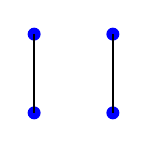
\begin{tikzpicture}
            \filldraw[blue] (0,0) circle (0.075cm);
            \filldraw[blue] (1, 0) circle (0.075cm);
            \filldraw[blue] (0, 1) circle (0.075cm);
            \filldraw[blue] (1, 1) circle (0.075cm);
            \draw[thick] (0,0) -- (0, 1);
            \draw[thick] (1, 0) -- (1, 1);
        \end{tikzpicture}
    \end{center}

    Each vertex in this graph has at degree at least 1, but clearly this graph is connected, and thus it is a direct counterexample. Now let's take a look at why this proof by induction does not work.

    The fundamental reason this proof fails is becuase our inductive step assumes that we build up the graph by inserting vertices in one by one, and connecting them to the main graph at each step. However, this does not have to be the case, and thus we arrive at a false conclusion.

    Another way to think about this is the fact that we are effectively \textit{forcing} the solution to be true by connecting each added vertex at every step, but this is not the only way to build a graph of $n+1$ vertices from $n$, thus leading to a logical fallacy.

\end{solution}
\pagebreak
\Question {Tournament}  

A \emph{tournament} is defined to be a directed graph such that for every pair
of distinct vertices $v$ and $w$, exactly one of $(v,w)$ and $(w,v)$ is an edge
(representing which player beat the other in a round-robin tournament).

Prove that every tournament has a Hamiltonian path. In other words, you can always
arrange the players in a line so that each player beats the next player in the
line.

\begin{solution}
    We prove this by induction. First, we specify that if player $a$ wins against player $b$, then we draw a directed arrow going from $b$ to $a$. We also assume no ties, since each vertex must be directed.

    \textbf{Base case:} $n = 2$. In a case with 2 people, one player wins against the other, so our Hamiltonian path is simply to start at the loser and walk along the edge towards the winner. 

    \begin{center}
        \begin{tikzpicture}
            \filldraw[blue] (0,0) circle (0.075cm) node[anchor=east, xshift=-0.25cm] {Player $A$};
            \filldraw[blue] (2,0) circle (0.075cm) node[anchor=west, xshift=0.25cm] {Player $B$};
            \draw[thick, -{Latex[scale=1.2]}] (2,0) -- (0,0);
        \end{tikzpicture}
    \end{center}

    So in this diagram, we assume without loss of generality that player $A$ won against player $B$, so our Hamiltonian path would be to walk from player $B$ to player $A$.

    \textbf{Inductive Hypothesis:} Assume that for a tournament of $n \geq 1$ people, that there exists a Hamiltonian path. Let's label the players $\{p_1, p_2, \dots, p_n\}$.

    Now we add a player to this group of $n$ people, call this player $P$. Notice that there are three possibilities: $P$ wins against everybody else, $P$ loses against everybody else, or $P$ wins some portion of their games. 

    If $P$ wins all their games, then it means that all vertices connected to $P$ point towards $P$. Thus, to draw our Hamiltonian path, we simply start at any player $p_i$ and end on another player $p_j$, then walk along the path from $p_j \to P$, which is guaranteed to exist since $P$ won all their games.

    If $P$ loses all their games, then it means that all vertices connected to $P$ point \textit{away} from $P$. To draw our Hamltonian path, we start at $P$ and walk along one of the edges to a player $p_j$, and follow the Hamiltonian path for our original group of $n$ people. 

    If $P$ loses some portion of their games, the same process applies: start at $P$, then walk along one of the edges from $P \to p_i$, then walk along the  Hamiltonian path of the original $n$ players. 

    Since in all cases there exists a Hamiltonian path, then we are done. $\blacksquare$.
\end{solution}
\pagebreak
\Question{Proofs in Graphs} 

\begin{Parts}

\Part On the axis from San Francisco traffic habits to Los Angeles traffic habits, Old California is more towards San Francisco: that is, civilized. In Old California, all roads were one way streets. Suppose Old California had 
$n$ cities ($n \geq 2$) such that for every pair of cities $X$ and $Y$,
either $X$ had a road to $Y$ or $Y$ had a road to $X$.

Prove that there existed a city which was reachable from every other city by traveling through at most 2 roads. 

[\textit{Hint:} Induction]

\begin{solution}
    We prove this by induction. 

    \textbf{Base case:} $n = 2$. If we have 2 cities, call them $X$ and $Y$. Then the road connecting the two either leads from $X \to Y$ or $Y \to X$. In either case, it's obvious that one of the two cities is reachable from the other by travelling through that road, and we are done. 


    \textbf{Inductive Hypothesis:} Assume that for $n$ cities, there exists one city that is reacahble from every other by travelling through at most 2 roads. We now prove that this is also the case for $n+1$ cities. 
    
    Suppose we have a graph of $n+1$ cities, and remove one node. Now, we have a graph of $n$ vertices, where there must exist one city (call it city $X$) that is reachable by travelling through at most 2 roads. 

    Now add the last city back, call this city $P$. Then, the connection of $P$ to $X$ can go in one of two directions. From $P \to X$ or from $X \to P$. If the connection is from $P \to X$, then we are done, since $X$ is reachable from $P$ using one road. 

    If the connection is from $X \to P$, look at the vertices that are 1 road away from $X$, and that point towards $X$. That is, these are the set of vertices $\{Y_1, \dots, Y_i\}$ such that they all have a road connecting $Y_i \to X$.
    
    If $X$ is reachable from 2 roads, then it follows that every $Y_i$ is reachable within 1 road. Now consider the roads connecting $Y_i$ and $P$. If the connection of one of these roads is $P \to Y_i$, then $X$ is reachable from $P$ within 2 roads. Otherwise, if all connections are $Y_i \to P$, then this means that every city is connected to $P$ within 2 roads, by travelling along the edge leading to $Y_i$ then travelling along $Y_i \to P$. Note that $X$ is also clearly connected to $P$ since the road between $X$ and $P$ is connected $X \to P$. $\blacksquare$
\end{solution}
\Part Consider a connected graph $G$ with $n$ vertices which has exactly $2m$ vertices of
odd degree, where $m > 0$. Prove that there are $m$ walks that \emph{together} 
cover all the edges of $G$ (i.e., each edge of $G$ occurs in exactly one of the $m$ walks, 
and each of the walks should not contain any particular edge more than once).

[\emph{Hint:} In lecture, we have shown that a connected undirected graph has an Eulerian tour if and only if every vertex has even degree. This fact may be useful in the proof.]

\begin{solution}
    Call the vertices with even degree $\{e_1, \dots, e_i\}$ Take a pair the vertices with odd degree, call them $u$ and $v$, and ``combine'' them. That is, construct a new vertex which is connected to all the vertices $u$ and $v$ are connected to. This new vertex is guaranteed to have an even degree, since it was constructed by combining two vertices of odd degree. We can do this $m$ times, since there are $2m$ \textit{pairs} of vertices with odd degree. Call these newly merged vertices $\{V_1, \dots, V_m\}$. Note that this is allowed since each vertex of odd degree is connected to one another, by definintion of a connected graph.

    Now, we have a graph of $n - m$ vertices, where each vertex has even degree. Now, we can construct $m$ walks as follows: start at one of the vertices $V_i$ and perform an eulerian walk between $V_i$ and a subset of vertices of even degree $e_i$. We do this $m$ times, one for each vertex $V_i$, which are our $m$ walks. 

    Now we need to prove that the walks will not interfere with each other. Since we start at $V_i$, we are guaranteed to never end on a vertex with even degree. Now let's analyze what happens when we traverse a through a vertex $e_i$: we are guaranteed to reduce its ``effective degree'' (i.e. the edges that have yet to be travelled) by an even amount, since for every time we enter an edge, we must exit it, thus reducing the number of edges by 2. Since the edges start out with an even degree, they must remain with an even degree. Thus, regardless of how we construct our Eulerian tours, one tour will not affect the other. As a result, we are done. $\blacksquare$
\end{solution}

\Part Prove that any graph $G$ is bipartite if and only if it has no tours of odd length.

[\emph{Hint:} In one of the directions, consider the lengths of paths starting from a given vertex.]

\begin{solution}
    We first prove that if a graph has is bipartite, then it has no tours of odd length. If a graph is bipartite, then this means that we can place each vertex into two sets $X$ and $Y$, such that traversing an edge means traversing from a vertex in set $X$ to set $Y$. 

    Now we prove by contradiction. Suppose there exists a bipartite graph with a tour of odd length. Now choose a vertex $v$ from this tour. Without loss of generality, let $v$ belong to set $X$. This is contradictory, since if we perform our walk of odd length we will end up with the conclusion that $v$ must be in $Y$. Since $v$ cannot be in both, we've reached a contradiction, and a tour of odd length cannot exist.

    Now we prove the reverse: if a graph has no tours of odd length, then the graph is bipartite. We can make a similar argument as the previous case. Since no tour of odd length exists, then if a tour does exist, it has an even length, and thus if a vertex belongs to set $X$ then it will remain in set $X$ after completing the tour. Since this is the case, we can alternately label every vertex on this tour to belong to set $X$ and $Y$, without issue. If a graph has no tours at all, then this is also true, since a tree (which contains no cycles, and thus tours) is guaranteed to be bipartite, as done in one of the discussion problems $\blacksquare$
\end{solution}
\end{Parts}
\pagebreak
\Question{Planarity and Graph Complements}

Let $G = (V, E)$ be an undirected graph.  We define the complement of $G$ as $\overline{G} = (V, \overline{E})$ where $\overline{E} = \{(i,j) \mid i,j \in V, i \neq j\} - E$; that is, $\overline{G}$ has the same set of vertices as $G$, but an edge $e$ exists is $\overline{G}$ if and only if it does not exist in $G$.

\begin{Parts}

\Part Suppose $G$ has $v$ vertices and $e$ edges.  How many edges does $\overline{G}$ have?


\begin{solution}
    There are ${v \choose 2} = \frac{v(v-1)}{2}$ possible edges in a graph of $n$ vertices. Thus, if $e$ of them are connected, then $\overline G$ will have $\frac{v(v-1)}{2} - e$ edges.
\end{solution}
\Part Prove that for any graph with at least 13 vertices, $G$ being planar implies that $\overline{G}$ is non-planar.

\begin{solution}
    In order for a graph to be planar, it must satisfy the relation:

    \[ e \leq 3v - 6\]

    So this must be true for a graph with larger than 13 vertices. If $G$ is planar, then it satisfies $e \leq 3(v - 2)$ so this means that $\overline G$ must have 

    \[ e' = \frac{v(v-1)}{2} - e\] 

    Now since $e$ is bouded above, then the minimum number of edges $\overline G$ must have is $\frac{v(v-1)}{2} - 3(v-2)$. To prove that $\overline G$ is not planar, we show the following inequality is true:

    \[ \frac{v(v-1)}{2} - 3(v-2) > 3(v-2) \implies \frac{v(v-1)}{2} > 6(v-2)\]

    for all $v \geq 13$. We can show this true by induction. 

    \textbf{Base case:} $v = 13$. We can verify this by plugging it in:

    \[\frac{13 \cdot 12}{2} = 78 > 66\]

    \textbf{Inductive Hypothesis:} Suppose this inequality holds for some $v \geq 13$. We show that this is also true for $v+1$. So we need to show:

    \[ \frac{v(v+1)}{2} > 6(v+1-2) = 6(v-1) \]

    Notice we can write the left hand side as 

    \[\frac{v(v+1)}{2} =x \frac{v(v-1)}{2} + v > 6(v - 2) + v\] 

    Simultaneously, we can rewrite $6(v-1) = 6(v-2) + 6$, and since $v \geq 13 > 6$ then $6(v-2) + v > 6(v-1)$, and thus our inductive step is done. As a result, our original inequality is true, which implies that $\overline G$ is guaranteed to be nonplanar if $G$ is planar, when $G$ has more than 13 vertices. $\blacksquare$.




\end{solution}

\Part Now consider the converse of the previous part, i.e., for any graph $G$ with at least 13 vertices, if $\overline{G}$ is non-planar, then $G$ is planar. Construct a counterexample to show that the converse does not hold.

\textit{Hint: Recall that if a graph contains a copy of $K_5$, then it is non-planar. Can this fact be used to construct a counterexample?}

    \begin{solution}
        We first show that the complement of $\overline G$ is in fact $G$. This is true because we know that edge $e$ exists in $\overline G$ if and only if it does not exist in $G$, then edge $e$ does not exist in the complement of $\overline G$. At the same time, $e$ could only exist in $\overline G$ if it had not existed in $G$. Since this is true for every edge, it follows that the complement of $\overline G$ is $G$.
        
        
        Suppose the following is $\overline G$:

        \begin{center}
            \begin{tikzpicture}
                \filldraw[blue] (0, 0) circle (0.075cm);
                \filldraw[blue] (0, 3) circle (0.075cm);
                \filldraw[blue] (-2.85, 3.93) circle (0.075cm);
                \filldraw[blue] (-4.62, 1.5) circle (0.075cm);
                \filldraw[blue] (-2.83, -0.93) circle (0.075cm);

                \filldraw[blue] (-7.1, 1.63) circle (0.075cm);
                \filldraw[blue] (-6.27, 4.22) circle (0.075cm); 
                \filldraw[blue] (-3.43, 5.7) circle (0.075cm);
                \filldraw[blue] (-0.24, 5.67) circle (0.075cm); 
                \filldraw[blue] (2.17, 3.84) circle (0.075cm);
                \filldraw[blue] (2.39, 1.57) circle (0.075cm);
                \filldraw[blue] (2.51, -1.03) circle (0.075cm);
                \filldraw[blue] (-1.04, -2.69) circle (0.075cm);
                \filldraw[blue] (-5.78, -2.11) circle (0.075cm);


                \draw[thick] (-4.62, 1.5) -- (-7.1, 1.63) -- (-6.27, 4.22) -- (-2.85, 3.93);
                \draw[thick] (-6.27, 4.22) -- (-4.62, 1.5);
                \draw[thick] (-7.1, 1.63) -- (-2.85, 3.93);

                % \draw[thick] (-7.1, 1.63) -- (-6.27, 4.22) -- (-3.43, 5.7) -- (-0.24, 5.67) -- (2.17, 3.84) -- (2.39, 1.57) -- (2.51, -1.03) -- (-1.04, -2.69)-- (-5.78, -2.11) -- cycle;
                % \draw[thick] (-7.1, 1.63) -- (-4.62, 1.5) -- (-6.27, 4.22) -- (-2.85, 3.93) -- (-3.43, 5.7) -- (0, 3) -- (-0.24, 5.67);
                % \draw[thick] (0, 3) -- (2.17, 3.84);
            \end{tikzpicture}
        \end{center}

        This graph has 13 vertices, and is nonplanar. Furthermore, $G$ also cannot be planar since the inner pentagon is a copy of $K_5$, which we know is nonplanar. We also know that the edges that connect this copy must exist in $G$, since they don't exist in $\overline G$. $\blacksquare$     
    \end{solution}


\end{Parts}
\pagebreak
\Question{Touring Hypercube} 

In the lecture, you have seen that if $G$ is a hypercube of dimension $n$, then
\begin{itemize}
    \item The vertices of $G$ are the binary strings of length $n$.
    \item $u$ and $v$ are connected by an edge if they differ in exactly one bit location.
\end{itemize}

A \emph{Hamiltonian tour} of a graph is a sequence of vertices
$v_0, v_1, \ldots, v_k$ such that:
\begin{itemize}
    \item Each vertex appears exactly once in the sequence.
    \item Each pair of consecutive vertices is connected by an edge.
    \item $v_0$ and $v_k$ are connected by an edge.
\end{itemize}

\begin{Parts}

    \Part Show that a hypercube has an Eulerian tour if and only if $n$ is even.
    
    \begin{solution}
        We prove the forward case: we show that a hypercube has an Eulerian tour if $n$ is even.

        In a hypercube, there are $2^n$ vertices, and $n2^{n-1}$ edges. Thus, if $n$ is even, then the number of edges that each vertex is connected to is $n$, since the number of places a bit can differ in exactly one location is $n$ locations. Since each vertex is connected to an even number of vertices, we know that an Eulerian tour exists. 

        We now show the reverse case: that if a hypercube has an Eulerian tour, then $n$ is even. We can use the same logic for this one as the previous direction: since a hypercube has an Eulerian tour, we know that each vertex is connected to an even number of vertices. Further, since we also know that each vertex is connected to $n$ vertices, then $n$ must be even. 

        Since both sides are complete, then we are done. $\blacksquare$
    \end{solution}
    \Part Show that every hypercube has a Hamiltonian tour. 

    \begin{solution}
        We only need to show this to be true for odd dimensions, since if the dimension is even, the previous part proves that an Eulerian tour exists, and thus so does a Hamiltonian tour. That said, the proof below handles both even and odd dimensions simultaneously:

        We prove this by contradiction. Suppose there exists a hypercube such that a Hamiltonian tour does not exist. Thus, this means there exists a vertex $v$ that is unreachable by a Hamiltonian tour. Since the hypercube must be connected, this means that all edges connected to $v$ have been traversed. But if this is the case, then this necessarily means that $v$ can be reached, since since the only way to traverse an edge connected to $v$ is to pass through $v$ or start at $v$, and in either case this means that vertex $v$ is reachable. Since $v$ cannot be both reachable and unreachable at the same time, we've arrived at a contradiction. Thus, a Hamiltonian tour always exists. $\blacksquare$
    \end{solution}

\end{Parts}
\pagebreak
\Question{Connectivity}

Consider the following claims regarding connectivity:
\begin{Parts}
    \Part  Prove: If $G$ is a graph with $n$ vertices such that for any two non-adjacent vertices $u$ and $v$, it holds that $\deg u + \deg v \ge n - 1$, then $G$ is connected. 

 
    
    [\textit{Hint:} Show something more specific: for any two non-adjacent vertices $u$ and $v$, there must be a vertex $w$ such that $u$ and $v$ are both adjacent to $w$.]


    \begin{solution}
        If $\deg u + \deg v \ge n-1$, then this means that combined, $u$ and $v$ are connected to a minimum of $n-1$ vertices. However, excluding $u$ and $v$, there are only $n-2$ vertices that $u$ and $v$ can connect to. Therefore, by the pigenhole principle, there must exist at least one vertex which is both connected by $u$ and $v$. Thus, $u$ and $v$ must be connected. Further, since this is true for any $u$ and $v$, then it follows that $G$ is connected. $\blacksquare$
    \end{solution}


    \Part  Give an example to show that if the condition $\deg u + \deg v \ge n - 1$ is replaced with $\deg u + \deg v \ge n - 2$, then $G$ is not necessarily connected.

    \begin{solution}
        Suppose we have the following graph: 
        \begin{center}
            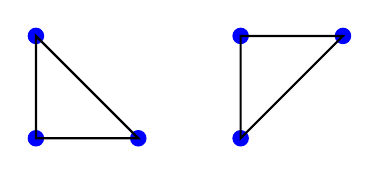
\begin{tikzpicture}[scale=1.3]
                \filldraw[blue] (0, 0) circle (0.075cm);
                \filldraw[blue] (1, 0) circle (0.075cm);
                \filldraw[blue] (0, 1) circle (0.075cm);
                \filldraw[blue] (2, 0) circle (0.075cm);
                \filldraw[blue] (2, 1) circle (0.075cm);
                \filldraw[blue] (3, 1) circle (0.075cm);
                \draw[thick] (0, 0) -- (0, 1) -- (1, 0) -- cycle;
                \draw[thick] (2, 0) -- (2, 1) -- (3, 1) -- cycle;
            \end{tikzpicture}
        \end{center}

        This graph has $n = 6$ vertices, and each pair of vertices $u$ and $v$ have $\deg u + \deg v = 4 \ge 6-2$, so the condition is satisfied, but clearly $G$ is connected. $\blacksquare$

    \end{solution}

    \Part Prove: For a graph $G$ with $n$ vertices, if the degree of each vertex is at least $n/2$, then $G$ is connected. 

    \begin{solution}
        We prove by contradiction. Suppose that there exists a graph $G$ such that each vertex has degree $n/2$ but the graph is not connected. As such, we are able to split the graph into two smaller graphs. Now we will handle the number of vertices in $G$ in two cases, based on parity: 

        \textbf{Case 1:} $G$ has an odd number of vertices. When we perform the splitting, we must split the graph into $\lfloor n/2 \rfloor$ and $\lceil n/2 \rceil$ vertices ($\lfloor x \rfloor$ and $\lceil x\rceil$ represent the floor and ceiling functions respectively). Now look at the graph with $\lfloor n/2\rfloor$ vertices. If each vertex has degree $n/2$, then this means that the graph should have at least $n/2+1$ vertices, which is impossible since $\lfloor n/2\rfloor < n/2 < n/2 + 1$.

        \textbf{Case 2:} $G$ has an even number of vertices. Now when we perform the splitting, we must split the graph into $n/2$ vertices each. However, this case fails by the same argument, since if each vertex must have degree at least $n/2$, then this implies that the minimum number of vertices in each smaller graph is $n/2+1$, which is a contradiction. 

        Now we need to show that $\lfloor n/2 \rfloor$ and $\lceil n/2 \rceil$ is the optimal splitting. This is easy to show, since if we add vertices to one of the two graphs, then we must take away from the other, and thus we are guaranteed to remain below $\lfloor n/2 \rfloor +1$ vertices in at least one of the graphs. 
        
        And thus, since both cases lead to a contradiction, $G$ must be connected, and we are done. $\blacksquare$
    \end{solution}
    
    \Part Prove: If there are exactly two vertices with odd degrees in a graph, then they must be in the same connected component (meaning, there is a path connecting these two vertices). 
    
    [\textit{Hint:} Proof by contradiction.]

    \begin{solution}
        As per the hint, we prove this by contradiction. Suppose we have a graph with two odd vertices but they are not connected by a path. Call these vertices $V_1$ and $V_2$. Then it follows from this that there is no vertex connected to $V_1$ that connected to $V_2$, and vice versa. Thus, the graphs containing $V_1$ and $V_2$ can equivalently be thought of as separate graphs. 

        If they are separate graphs, then they must obey the property that $\sum_{v \in V} \deg v = 2|E|$. But since each graph only contains one node with an odd number of vertices, this sum cannot be odd, and thus we've arrived at a contradiction. Therefore, if there are exactly two vertices with odd degrees in a graph, then they must be in the same connected component. $\blacksquare$
    \end{solution}
\end{Parts}
\pagebreak 
\Question{Edge Colorings}

An edge coloring of a graph is an assignment of colors to edges in a graph where any two edges incident to the same vertex have different colors. An example is shown on the left.

\begin{center}
    \begin{tikzpicture}
        \clip (-1, -1) rectangle (8, 2.1);

        \node[circ] (n1) at (0, 0) {};
        \node[circ] (n2) at (1, {sqrt(3)}) {};
        \node[circ] (n3) at (2, 0) {};
        \draw (n1) -- node[above left] {color 1} (n2)
        -- node[above right] {color 2} (n3)
        -- node[below] {color 3} (n1);

        \node[circ] (m1) at (5, 0) {};
        \node[circ] (m2) at (5, 2) {};
        \node[circ] (m3) at (7, 2) {};
        \node[circ] (m4) at (7, 0) {};
        \draw (m1) -- (m2) -- (m3) -- (m4) -- (m1);
        \draw (m2) -- (m4);
        \draw (m1) edge[out=-60, in=-30, looseness=2.5] (m3);
    \end{tikzpicture}
\end{center}

\begin{Parts}
\Part Show that the 4 vertex complete graph above can be 3 edge colored. (Use the numbers $1,2,3$ for colors. A figure is shown on the right.)

\begin{solution}
    We can colour the graph as follows: 

    \begin{center}
        \begin{tikzpicture}
            \node[circ] (m1) at (5, 0) {};
            \node[circ] (m2) at (5, 2) {};
            \node[circ] (m3) at (7, 2) {};
            \node[circ] (m4) at (7, 0) {};
            \draw[green] (m1) -- (m2);
            \draw[purple] (m2) -- (m3);
            \draw[green] (m3) -- (m4);
            \draw[orange] (m2) -- (m4);
            \draw[orange] (m1) edge[out=-60, in=-30, looseness=2.5] (m3);
        \end{tikzpicture}
    \end{center}

    Where we've used three colours: green, purple and orange.
\end{solution}

\Part Prove that any graph with maximum degree $d \geq 1$ can be edge colored with $2d-1$ colors. 

\begin{solution}
    We prove this by contradiction. Suppose there exists a graph $G$ which has a maximum degree $d$, and it cannot be edge colored with $2d - 1$ colors. Thus, this means there exists a vertex $v$ such that $\deg v > 2d-1$, which is impossible since this vertex has degree $d \le 2d -1$ (with equality at $d=1$), and we've arrived at a contradiction. Therefore it is always possible to colour a graph with maximum degree $d \ge 1$ with $2d-1$ colours. $\blacksquare$
\end{solution}

\Part Show that a tree can be edge colored with $d$ colors where $d$ is the maximum degree of any vertex.

\begin{solution}
    We prove via induction on $d$.

    \textbf{Base case:} If the maximum degree of any vertex in the tree is 1, then this means that this tree consists of a root and leaf node. Clearly, we only need one colour for this tree, since there is only one edge to be coloured.

    \textbf{Inductive Hypothesis:} Assume that a tree with maximum degree $d$ can be coloured with $d$ colours. Now we prove the statement is true for a tree with maximum degree $d+1$.

    Take all vertices that have degree $d+1$, and remove a vertex from them. If all vertices connecting a vertex of degree $d+1$ also has degree $d+1$, remove one vertex from those as well. After this process, the maximum degree that this tree has is degree $d$, which we know is colourable with $d$ colours. 

    Now we add back the removed vertices. When connecting these vertices back to the main tree, we can use the unused colour (since there are $d+1$ colours in total) to colour in these newly formed edges. Furthermore, since this colour was unused until the additino of these nodes, then there cannot possibly be an interfering edge, and thus a tree with maximum degree $d+1$ is colourable using $d+1$ colours. $\blacksquare$
\end{solution}

\end{Parts}

\end{document}
